\chapter{Theoretical introduction}
\minitoc
This thesis presents the measurement of a Standard Model (SM) process, so the first section of this chapter gives a small overview of the Standard Model. Since this thesis uses data collected in proton-proton collisions, the proton structure (Sec.~\ref{sec:ProtStr}) and physics of W and Z bosons in proton collisions (Sec.~\ref{sec:TheoWZ}) are discussed. Additionally, the predictions for $W\to l\nu$ and $Z \to ll$ cross-sections are presented in the last section.

A variety of sources were used for a preparation of this chapter, including \cite{QPrim, Okun}.
\section{Standard model}

The Standard Model (SM) is the the theory, that explains the fundamental elementary particles and their interactions. It provides our best understanding of the particle physics and unifies the quantum mechanichs, special relativity and a field theory. It was postulated by Weinberg-Salam in mid-1970\cite{SM1, SM2, SM3} and was successfully tested for the last 40 years. Despite the fact, that there are some unexplained phenomena in SM, such as dark matter and gravitation, it describes almost all laboratory data. The summary of all standard model cross-section measurements at \atlas experiment is given in Fig.~\ref{fig:SMxsec}. The results are agreeing with SM over several orders of magnitude and no significant deviation from SM has been found yet.

\begin{figure}[!tpb]
\center{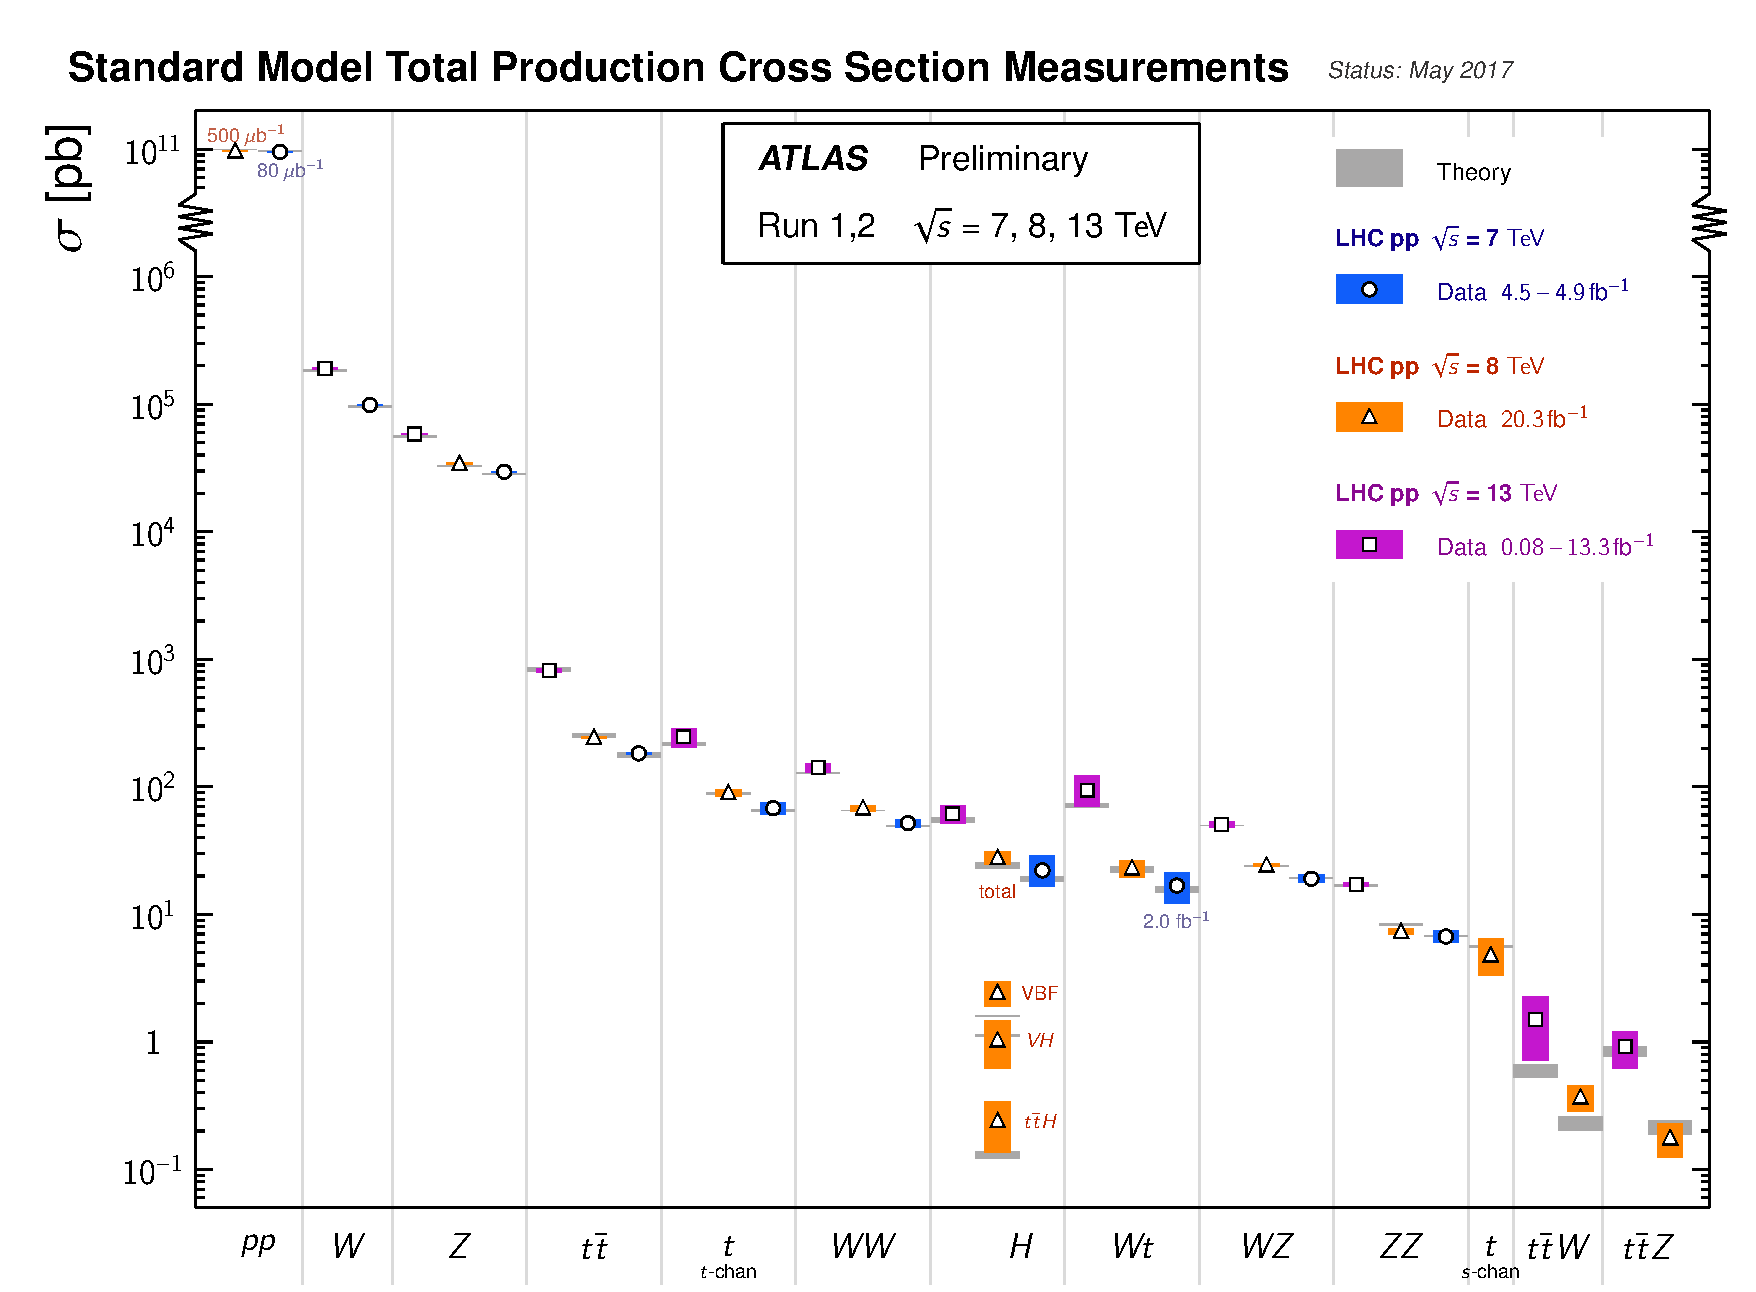
\includegraphics[width=0.9\linewidth]{Theory/SMXsec.pdf} }
\caption{Summary of several Standard Model total production cross section measurements, corrected for leptonic branching fractions, compared to the corresponding theoretical expectations. All theoretical expectations were calculated at NLO or higher. The luminosity used for each measurement is indicated close to the data point \cite{SMPubRes}}
\label{fig:SMxsec}
\end{figure}

The SM postulates two types of fundumental particles: fermions and boson. Graphical representation of particles in SM with their masses and quantum numbers is shown in Fig.~\ref{fig:SMPart}. The fermions are the spin 1/2 particles that form the matter. They can be further divided to leptons and quarks. Leptons can interact just electromagnetically and weakly, while quarks undergo strong and electroweak interactions. Both groups are divided into 3 separate generations.

\begin{figure}[!tbp]
\center{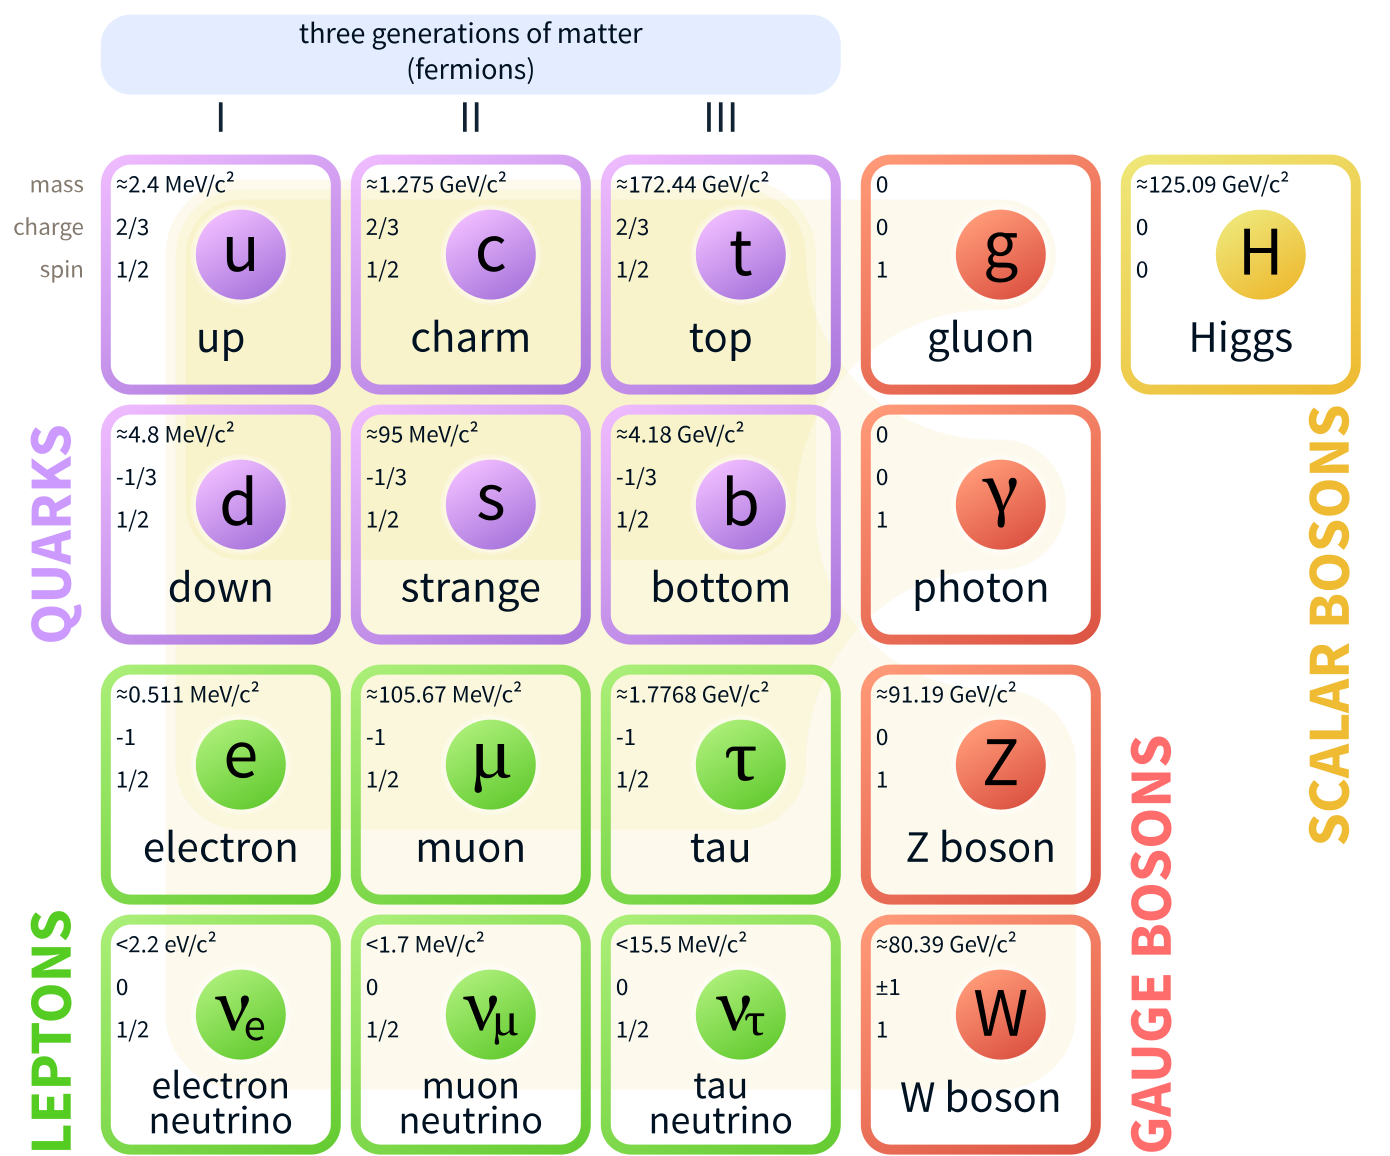
\includegraphics[width=0.5\linewidth]{Theory/SM.png} }
\caption{All fundamental particles of the Standard Model with three generations of matter, the gauge and Higgs bosons \cite{SMParticles}}
\label{fig:SMPart}
\end{figure}

The bosons are the carriers of the fundamental forces with the integer spin. Strong interactions are mediated by 8 massless gluons. The massless photons are carrying the electromagnetic interactions, while the W and Z bosons are responsible for the weak forces. The last SM boson, observed in experimental data is the Higgs boson\cite{HiggsDiscoATLAS, HiggsDiscoCMS}. It is assosiated with Yukawa interactions, that are responsible for the fermion masses. 

The SM is a \textit{non-abelian gauge theory}, that means, that this theory is based on an invariant under local and global transformations (called \textit{symmetries}) Lagrangian. From the Noether theorem\cite{Noether1, Noether2} it is known, that each symmetry is connected to at least 1 conserved quantity. The symmetry group of SM is:
\begin{equation}
SU(3)_C \times SU(2)_L \times U(1)_Y,
\end{equation}
where Y a hypercharge, L - a left-handed helicity and C a color charge - are the conserved values of the corresponding symmetry group. The  $SU(2)_L \times U(1)_Y$ symmetry stands for quantum electrodynamics (QED), while the $SU(3)_C$ corresponds to the theory of strong interactions - Quantum Chromodynamics (QCD)\cite{QCD1, QCD2, QCD3}. 

The QED postulates three massless vector fields in $SU(2)_L$ - the isospin triplet of vector fields $W^1_\mu$, $W^2_\mu$, $W^3_\mu$ with the coupling constant $g$ and a single gauge field $B_\mu$ in $U(1)_L$ group with coupling strength $g'$. The actual $\gamma$ and the massive Z and W bosons are produced due to the spontaneous breaking of the electroweak gauge symmetry as:
        \begin{align}
                \left(\gamma \atop Z^0 \right)
                &= \left(
            \begin{array}{cc}
            \cos \theta_W & \sin \theta_W \\
            -\sin \theta_W & \cos \theta_W
            \end{array}
            \right)
                \left(B \atop W^3 \right)
                 \\
                 W^\pm& = \frac{W^1 \pm i W^2}{\sqrt{2}},
        \end{align}
where  $\theta_W$ is the electroweak mixing angle which value is not predicted in the theory. The masses of Z and W bosons are connected by the relation:
\begin{equation}
M^2_W=cos^2_W M^2_Z
\end{equation}


The QCD Lagrangian has only one pararameter - a \textit{strong coupling constant} $\alpha_s$. QCD theory uses a concept  similar to QED, however it is more complicated because of the color charge of qluons, that allows them to interact with each other. The inclusion of the gluon-gluon interaction causes a  \textit{ultraviolet} (UV) divergences in the corresponding integrals. The renormalization procedure\cite{Renorm} allows to move them into the coupling constant by introducing the arbitrary renormalization scale $\mu_R$. A typical scale for a physics process corresponds to the momentum transferred $Q^2$. 

The QCD does not predict the value of $\alpha_s$, however it can predict its evolution with renormalization scale using the renormalization group equation (RGE):
\begin{equation}
\beta(\alpha_s) = \mu^2 \frac{d\alpha_s(\mu^2)}{d\mu^2}= - b_0 \alpha_s^2(\mu) - b_1 \alpha_s^3(\mu)-..., 
\end{equation}
where the first coefficient is:
\begin{equation}
b_0 = \frac{33-2f}{12\pi},
\end{equation}
where f=3 is the number of flavors. This leads to energy dependence of the coupling constant showed in Fig.~\ref{fig:SMAlphaS} together with results, obtained in experiments. The coupling constant increases with smaller scales, but becomes small for higher $Q^2$. As a consequence, the quarks have a property of \textit{asymptotic freedom} and \textit{confinement}, meaning that they cannot be observed as free particles, but are almost not interacting in a bound state, like a proton.

\begin{figure}[!tbp]
\center{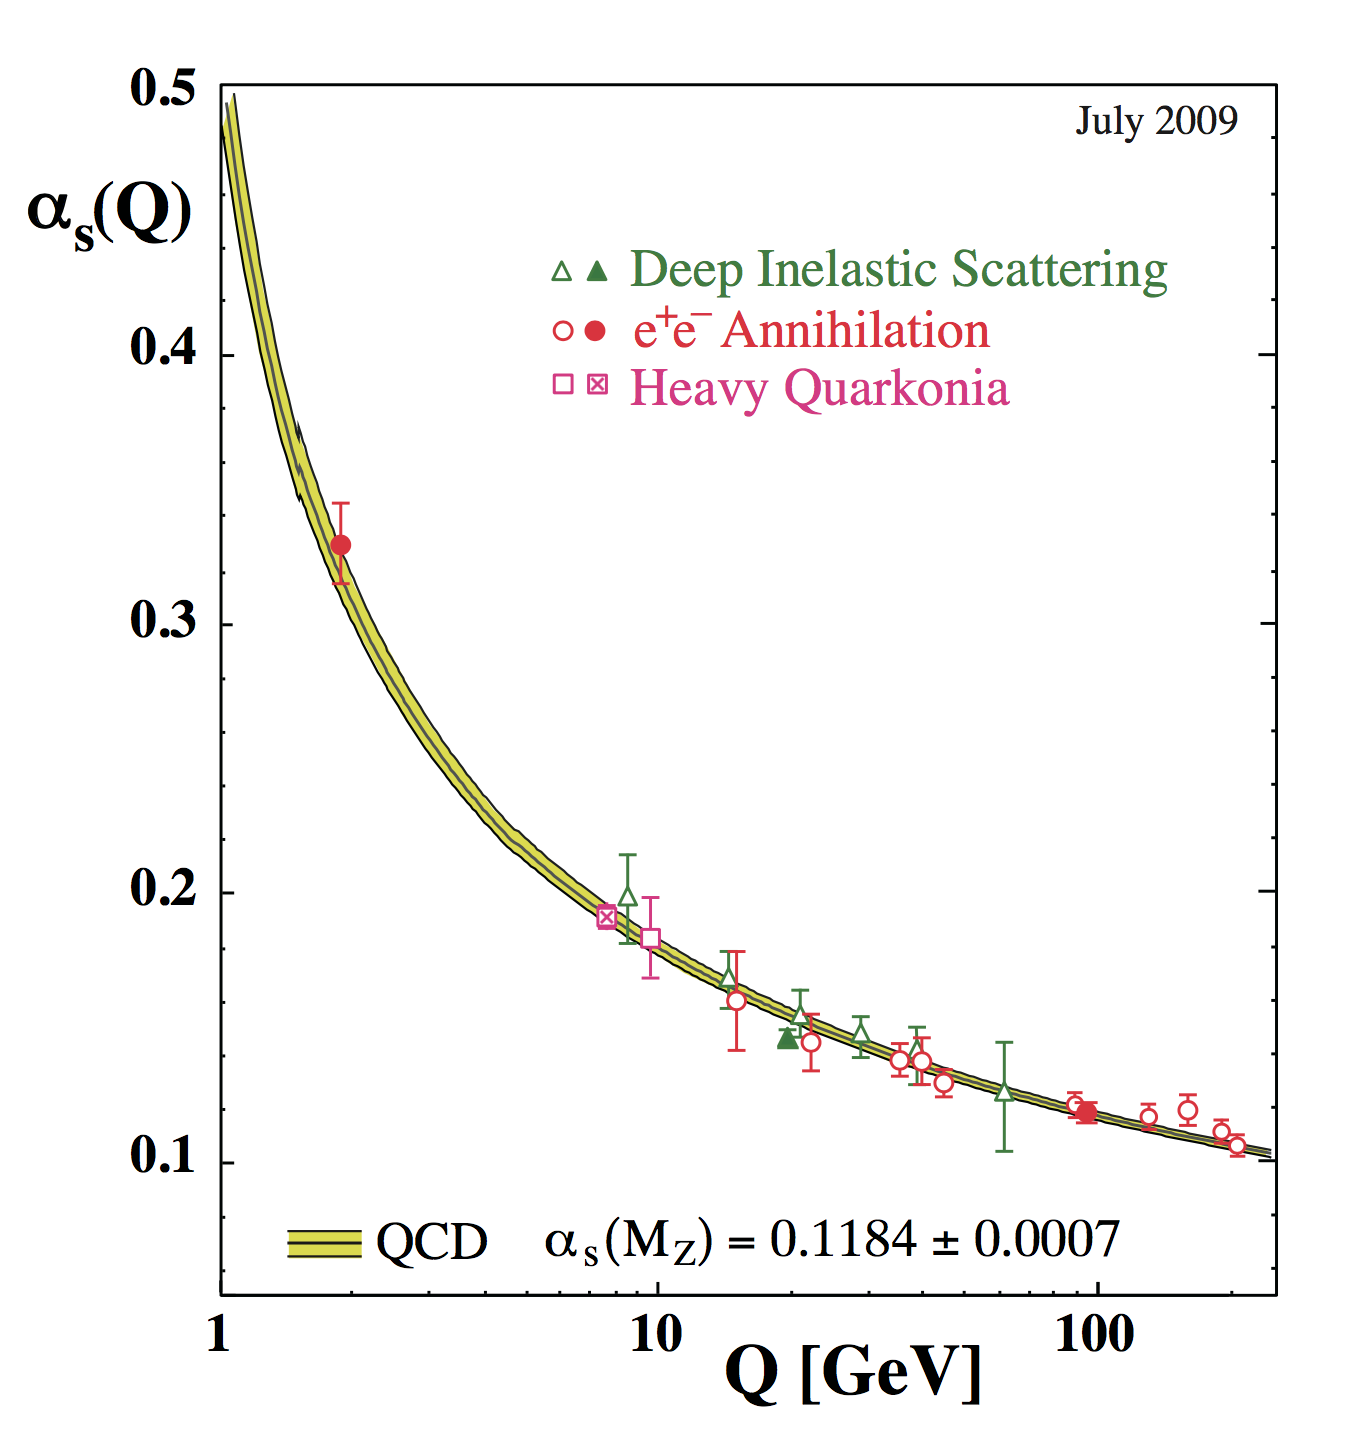
\includegraphics[width=0.5\linewidth]{Theory/alphaS.png} }
\caption{The coupling $\alpha_s$ of the strong interaction as a function of energy scale \cite{alphaS}}
\label{fig:SMAlphaS}
\end{figure}


The full physical quantities do not depend on renormalization scale, however, the calculation on any pertrubative order is a function of $\mu_R$. The cross-section of the partonic interaction (or the \textit{partonic cross-section}) $\sigma_{ab\to X}$ can be expressed pertrubativelly in orders of $\alpha_s$ as:
\begin{equation}
\sigma_{ab\to X}=\hat{\sigma_0}+\alpha_{s}(\mu_R)\hat{\sigma_0}+\alpha^2_{s}(\mu_R)\hat{\sigma_2}+..., 
\end{equation}
where $\sigma_i$ are the i-th order contributions to the final cross-section. The cross-section, calculated at lowest order of the expansion is called the \textit{leading order} (LO) cross-section. The calculation using the expansion of $\alpha_s$ up to the i-th order is called (next to)$^i$ order (N$^i$LO) cross-section, there "next-to" (N) is repeated i times. The inclusion of higher order corrections allows to reduce the dependency on the renormalization scale. 


\section{Proton structure}\label{sec:ProtStr}
The cross-section of individual quark-quark interactions is predicted in QCD at the different orders of $\alpha_s$. However, since the quarks haven't been observed in a free state, the test of QCD predictions is possible only using the experiments with hadrons (e.g. proton beams), so the internal quark compostion in the hadron should be taken into account. 

Richard Feynman proposed  model of the proton structure called a parton model of the hadrons in 1969 \cite{Feynman1969}. In this model it is assumed, that any hadron can be treated as a composition of point-like constituents called partons. In the high momentum scattering the soft interaction between partons can be neglected, and therefore they can be treated as quasi free in collision. In this approximation of incoherent scattering a total cross-section for process in a hadron-hadron interaction could be written as a sum of all partonic cross-sections:
\begin{equation}
\sigma = \int dx_1 dx_2 f_1^{(P_1)}(x_1) f_2^{(P_2)}(x_2) \hat{\sigma}(x_1x_2s), 
\end{equation}
where:
\begin{itemize}
\item $f_1^{(P_1)}(x_1)$ and $f_2^{(P_2)}(x_2)$ are the parton distribution functions (PDF) for both colliding hadrons. It describes the probability to find parton i  in hadron j with a fraction of longitudial momentum $x_i$.
\item $\hat{\sigma}(x_1x_2s)$ is the partonic cross-section for a given scattering process, calculated in QCD.
\end{itemize}

The partons, which determine the quantum numbers of hadron, are called \textit{valence quarks} (u and d quarks in case of the proton).  However, due to the fluctuations, the infinite number of quark pairs of $u\bar{u}$, $d\bar{d}$, $c\bar{c}$ etc with low momentum could be created. These quarks are called \textit{sea-quarks}. Due to the conservation of the total momentum and the flavor of a proton, the following sum rules are applicable for proton PDFs:
\begin{center}
$\int_0^1dx \sum_i x f_i^{(p)}(x) = 1$\\
$\int_0^1dx (f_u^{(p)}(x)-f_{\bar{u}}^{(p)}(x)) = 1$\\
$\int_0^1dx (f_d^{(p)}(x)-f_{\bar{d}}^{(p)}(x)) = 1$\\
$\int_0^1dx (f_s^{(p)}(x)-f_{\bar{s}}^{(p)}(x)) = 1$\\,
\end{center}
where index i runs over the quark flavors.

For the partonic cross-sections, the soft emmision of real and virtual gluons causes a collinear singularities that do not cancel. However, it is possible to include intial state emisions below a given scale into non-perturbative parton distribution functions.  The cutoff parameter in this procedure is called a \textit{factorisation scale} $\mu_F$. This definition of PDFs is universal, i.e. does not depend on a physics process. Similarly to renormalization scale, the factorization scale $\mu_F$ is not a physical quantity and the total partonic cross-section should be independent independent of it. The typical choice of the factorization scale is $\mu_R \approx \mu_R \approx Q^2$.

These distributions cannot be calculated pertrubativelly in QCD and therefore need to be obtained from the data. However, it is possible to predict the evolution of PDFs with factorisation scale in pertrubative order using the DLGAP evolution equations \cite{Gribov:1972ri}. An example of quark and gluon PDFs predicted by MMHT2015 NNLO\cite{MMHT} for different scales are shown in Fig. \ref{fig:PFSMMHT}. The PDFs of valence u and d quarks are peaking at x=1/3, while the sea quark and gluo densities are rising at low x. The contribution of the sea quarks becomes larger with increasing $Q^2$.

\begin{figure}[!tbp]
\center{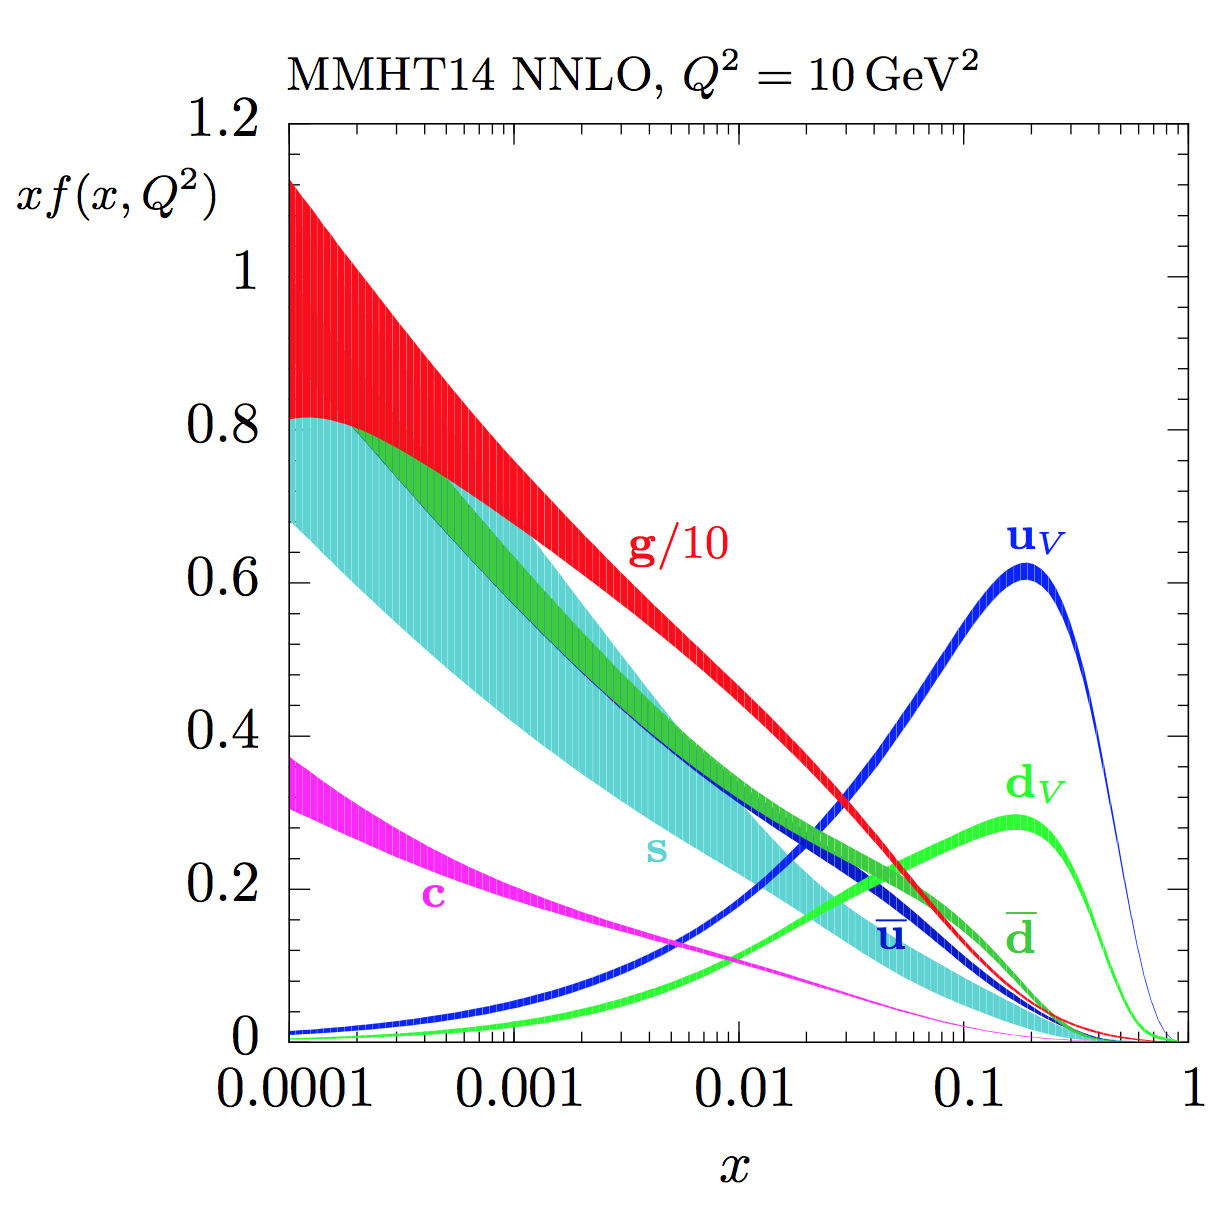
\includegraphics[width=0.9\linewidth]{Theory/MMHTPdfs.png} }
\caption{The MMHT2014 NNLO PDFs predictions at $Q^2 = 10 GeV^2$(left) and $Q^2 = 10^4 GeV^2$ (right), with associated 68\% confidence-level uncertainty bands.\cite{MMHT}}
\label{fig:PFSMMHT}
\end{figure}

\section{Physics of W and Z bosons in pp collisions}\label{sec:TheoWZ}

As it was mentioned the W and Z bosons are the vector bosons in Standard Model.
They have been predicted by the Glasgow, Weinberg, Salam un 1960's and discovered in 1983 by UA1 and UA2 at CERN $p\bar{p}$ collider\cite{Wdisc1, Wdisc2, Wdisc3, Wdisc4}.  These particles are mediating weak interactions and decaying almost immidiatly ($t \approx 10^{-25}$ s). 

The leading algorithm of their production is a Drell-Yan mechanism, shown schematically in Fig. \ref{fig:DY}. The Drell-Yan process is the process of production of lepton pair with 4-momentum $p_1$ and $p_2$ and large invariant mass $M_{ll}=\sqrt{(p_1^l +p_2^l)^2}$ in quark-antiquark annihilation. A simpliest example of this process is the production of the virtual photon $q\bar{q} \to \gamma^{*} \to l^+ l^-$. The corresponding cross-section can be calculated from fundamental  QED as:
\begin{equation}
\hat{\sigma}(q\bar{q} \to \gamma^{*} \to e^+ e^-) = \frac{4\pi\alpha}{3\hat{s}}\frac{1}{N}Q^2_q,
\end{equation}
where $Q_q$ is the quark charge, $\hat{s}$ is the centre of mass energy of quark-antiquark system and 1/N=1/3 is the overall color factor, coming from the fact, that quark and antiquark colors should match each other in order to create a colour-singlet in a final state.

\begin{figure}[!tbp]
\center{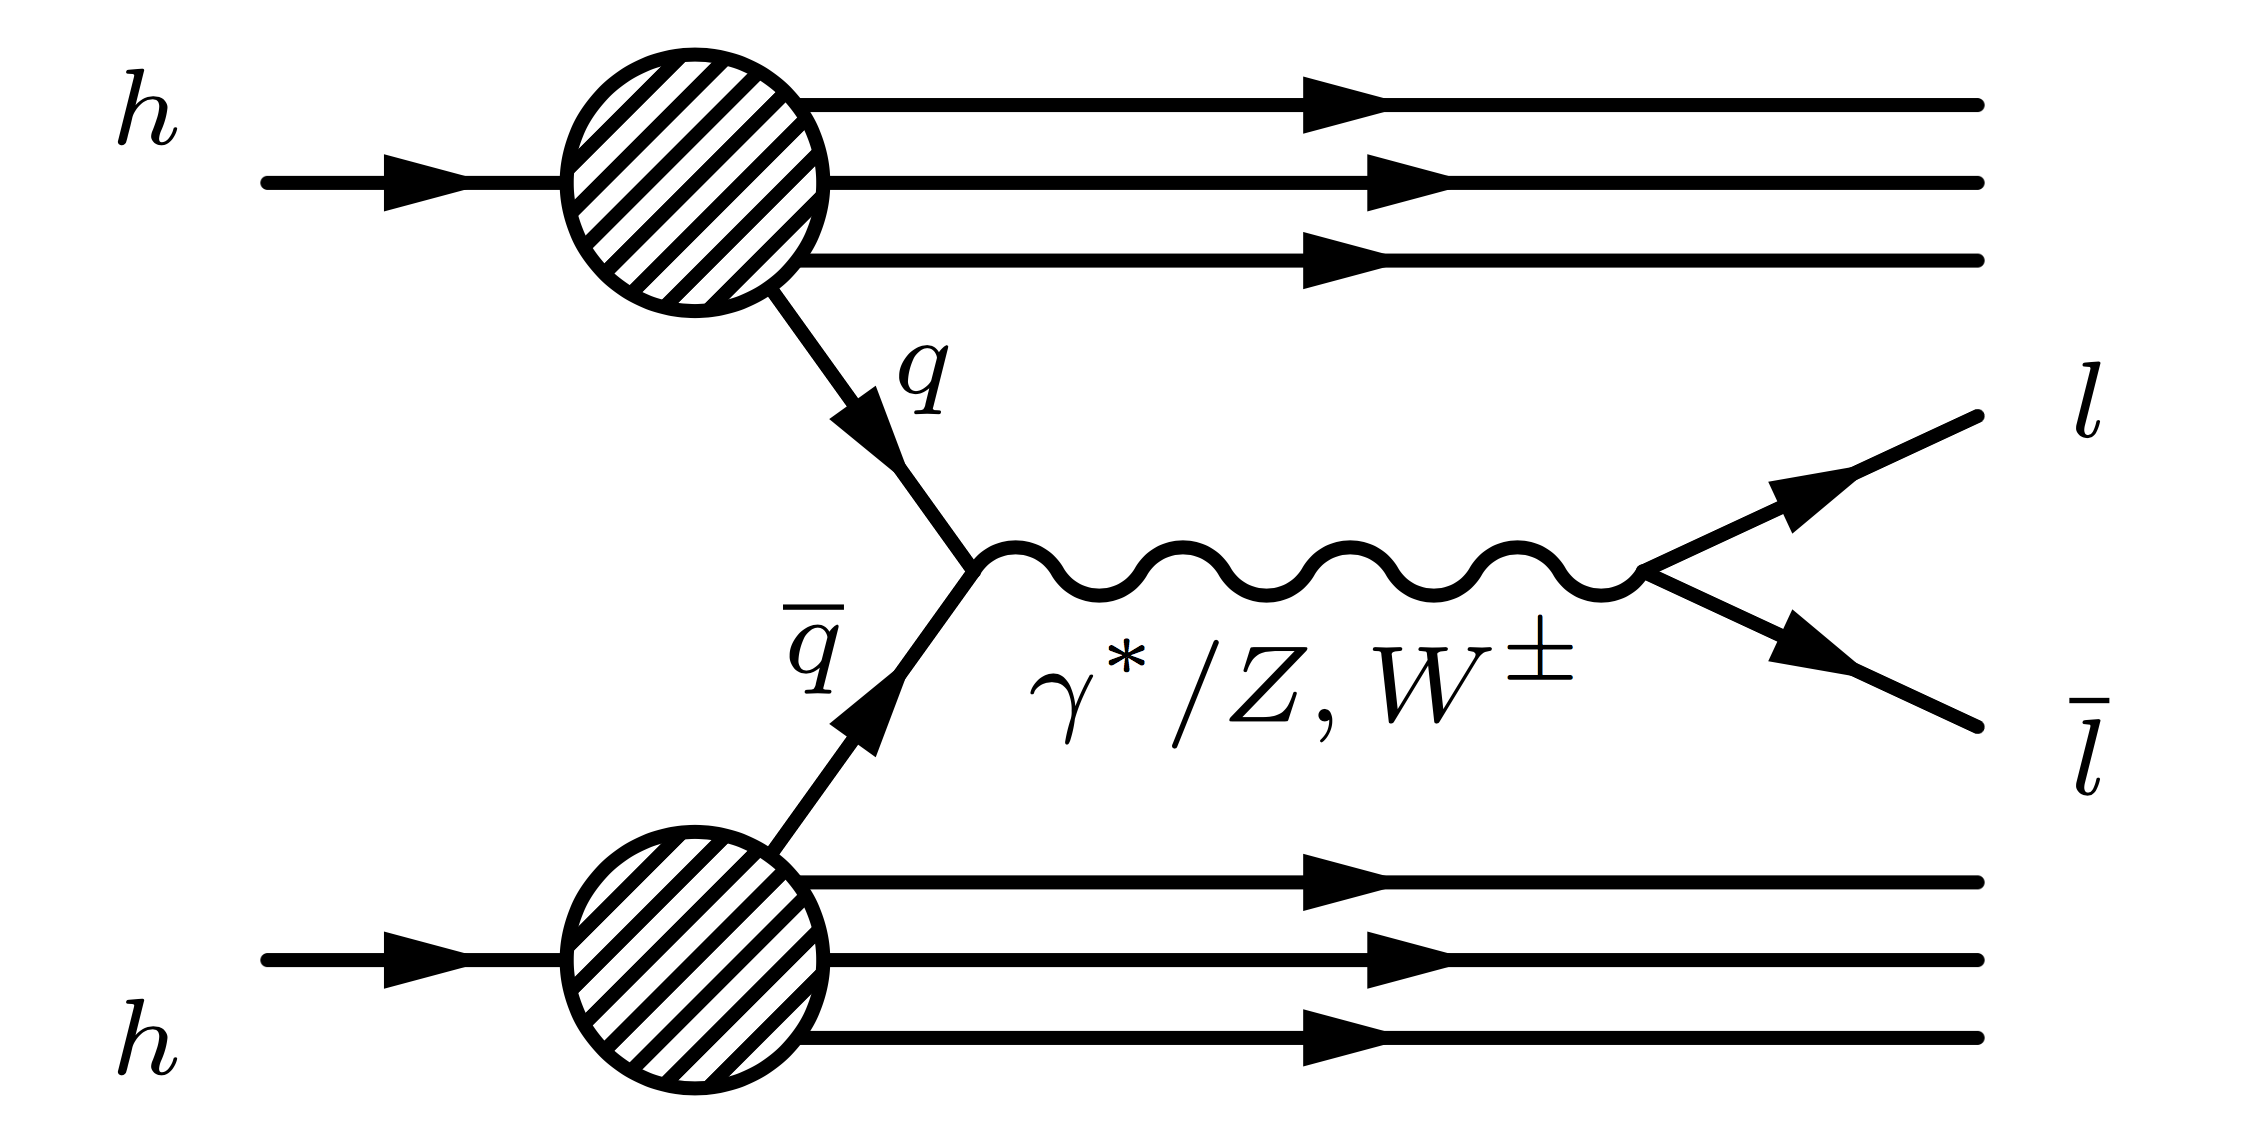
\includegraphics[width=0.7\linewidth]{Theory/DY.png} }
\caption{A schematic representation of the W/Z production via Drell-Yan process in a hadron collider.}
\label{fig:DY}
\end{figure}

In analogy to this process, the on-shell production of W and Z bosons with Drell-Yan process can be calculated as:
\begin{equation}
\hat{\sigma}^{q\bar{q}' \to W} = \frac{\pi}{3}\sqrt{2}G_F M^2_W | V_{q\bar{q}'}|^2 \delta (\hat{s}-M^2_{W}),
\end{equation}
\begin{equation}
\hat{\sigma}^{q\bar{q} \to Z} = \frac{\pi}{3}\sqrt{2}G_F M^2_Z (v^2_q+a^2_q) \delta (\hat{s}-M^2_{Z}),
\end{equation}
where the $q$ and $q'$ are the different quarks. The $V_{q\bar{q}'}$ is the appropriate Cabibbo-Kobayashi-Maskawa matrix element, what describes a strength of flavor changing weak decays, and $v_q$ ($a_q$) the vector (axial vector) coupling of the Z to the quarks. For the full production cross-section, the partonic spectrum of colliding hadrons should be considered. For 2 quarks, carrying fractions $x_1$ and $x_2$ of the protons momenta, the momentum transfer $Q^2$ can be written as:
\begin{equation}\label{eq:Q2}
Q^2 = (x_1p_1 + x_2p_2) \approx x_1 x_2 \sqrt{s} = M^2_{Z,W,\gamma^{*}},
\end{equation}
where the parton masses have been neglected in the calculation,  $s$ in the Eq.~\ref{eq:Q2} is the center-of-mass energy of 2 hadrons:
\begin{equation}
s=(p_1+p_2)^2.
\end{equation}


Another Lorentz invariant, used to describe the parton scattering is the rapidity of the boson, defined as:
\begin{equation}
y = \frac{1}{2} log \frac{E+P_z}{E-P_z},
\end{equation}
where $E$ is the energy of the boson and $P_z$ is the z component of the momentum.
This quantity can be connected to the momentum fraction carried by initial partons in a leading order approximation as:
\begin{equation}
x_{1,2}=\frac{M_{Z,W,\gamma}e^{\pm y}}{\sqrt{s}}.
\end{equation}
The maximum accessible rapidity range for the production of the bosons can be determined from the center-of-mass energy and the mass of the boson as:
\begin{equation}
|y^{max}_{bos}| = ln \frac{\sqrt{s}}{M_{bos}}.
\end{equation}

\begin{figure}[!tb]
\center{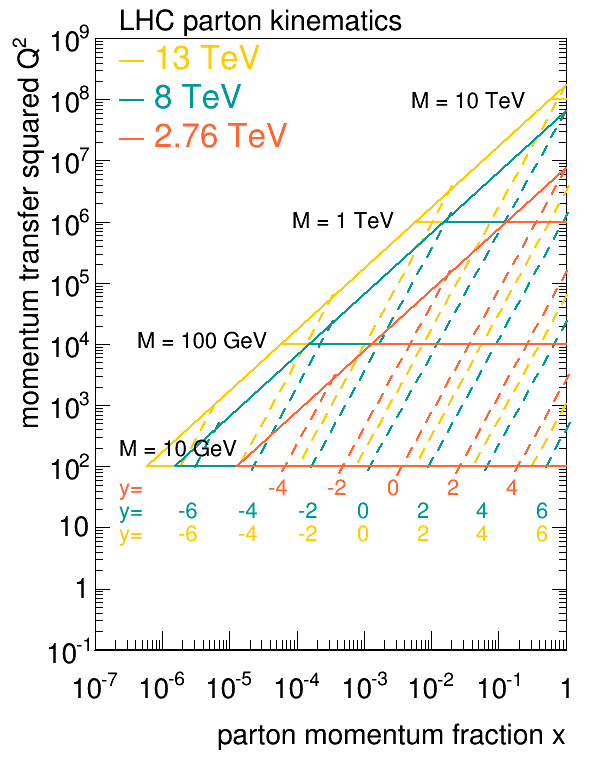
\includegraphics[width=0.5\linewidth]{Theory/LHCpartonkinematics.png} }
\caption{The LHC parton kinematics in $Q^2$ x plane. The LHC experiment limits are shown at $\sqrt{s}$ = 13 TeV, 8 TeV and 2.76 TeV.}
\label{fig:PartKin}
\end{figure}

The full parton kinematic phase-space, accessible at LHC for a different center-of-mass energies is shown in Fig.~\ref{fig:PartKin}. The W and Z cross-sections at 2.76 TeV correspond to $Q^2\approx 10^4 GeV^2$ and therefore can probe the ranges of partons fractions $x^{W}>8\cdot 10^{-4}$ and $x^{Z}>1 \cdot 10^{-3}$  for W and Z bosons respectively.  The $W^{+}$ production depends mainly on the $u$ and $\bar{d}$ distributions (because of the leading order process $u\bar{d}\to W^+$), the $W^{-}$ oppositely to $\bar{u}$ and $d$ distributions. The Z boson production cross-section is mostly sensitive to the valence quark distributions.

The Drell-Yan process contributes to around 65\% of the total production cross-section \cite{Ellis:318585}, with both valence-sea and sea-sea quarks interactions included. The dominant higher order cross-section  correction is the interaction of a quarks with a gluon, that occurs in approximately 20\% of the events. 

Due to the small time of life of W and Z bosons, the production is instantly followed by a decay. 
The probability of a certain decay mode is described by the \textit{branching ratio}, $\textbf{BR}(X\to a+b)$, that is a fraction of a partial decay rate of the decay mode of interest and the total decay rate of the boson.  The different decay modes are summarized in Tab. \ref{tab:WZDecayModes}. The W and Z bosons can decay hadronically with production of fermion-antifermion pair for all fermions, except for top quark, in case of the W boson, since its mass exceeds the mass of W.  This mode of the decay is the dominant one because of the 3 possible color states for each quark. In a leptonic decay of the W boson the lepton plus corresponding same flavor neutrino/antineutrino  pair is produced. The leptonic decays of Z create a lepton-antilepton pair. The visible fraction of Z bosons decaying into leptons is smaller, compared to W, because of the invisible mode of Z decay, where neutrino-antineutrino pair is produced.

\begin{table}[!tbp]
\begin{center}
\caption{Branching ratios of the different W and Z decay modes \cite{Agashe:2014kda}. Invisible denotes the Z decays with a neutrino-antineutrino pair as a final state. The predicted values are estimated with sin$^2\theta_W = 0.23$.}
\label{tab:WZDecayModes}
\begin{tabular}{l | c | c | c }
\hline
Boson & Decay mode & Measured & SM \\
	& & branching ratio & prediction \\
\hline
$W$ & $e\nu_e$ & $(10.71\pm0.16)\%$ & \\
    & $\mu\nu_{\mu}$ & $(10.63\pm0.15)\%$ & 11.1\% \\
    & $\tau \nu_{\tau}$ & $(11.38\pm0.21)\%$ & \\
    & hadrons & $(67.41\pm0.27)\%$& 66.7\% \\
 \hline
 $Z$ & $e^+e^-$ & $(3.363\pm0.004)\%$ & \\
 	& $\mu^+\mu^-$ & $(3.366\pm0.007)\%$ & 3.4 \% \\
 	& $\tau^+ \tau^-$ & $(3.3658\pm0.008)\%$ & \\
 	& invisible & $(20.00\pm0.06)\%$ & 20.5\% \\
 	& hadrons & $(69.91\pm0.06)\%$ & 69.2\% \\
 \hline 
\end{tabular}
\end{center}
\end{table}

Due to experimental difficulty to measure the hadronic decays, the  W/Z cross-sections are usually measured through their leptonic decays. The expected NNLO production cross-sections times their branching ratios estimated using FEWZ program\cite{FEWZ} and CT14nnlo\cite{CT14}, at 2.76 TeV are:
\begin{equation}\label{eq:WcsNNLO}
\sigma^{NNLO}_{W^+ \to l \nu} = 2114^{+8}_{-11}(scale)^{+57}_{-59}(PDF) [pb]
\end{equation}
\begin{equation}
\sigma^{NNLO}_{W^- \to l \nu} = 1265^{+5}_{-6}(scale)^{+32}_{-38}(PDF) [pb]
\end{equation}
and 
\begin{equation}\label{eq:ZcsNNLO}
\sigma^{NNLO}_{Z^- \to ll} = 304^{+1}_{-1}(scale)^{+7}_{-7}(PDF) [pb],
\end{equation}
where the the first uncertainty comes from the uncertainty of the scale $Q^2=M_{bos}^2$. The second uncertainty arises from the imperfect knowledge of proton PDFs. The difference between $W^{+}$ and $W^{-}$ cross-sections (called chare assymetry) is due to  the higher probability of finding a $u_v$ quark rather than $d_v$ quark in protons.

The NNLO predictions of W and Z cross-sections in $pp$ and $p\bar{p}$ collisions and results obtained at different experiments are shown in Fig.~\ref{fig:Wcs}-~\ref{fig:Zcs}. It can be seen, that the W and Z cross-sections have not been measured so far in region around 3 TeV in proton-proton collisions.


\begin{figure}[!tbp]

\center{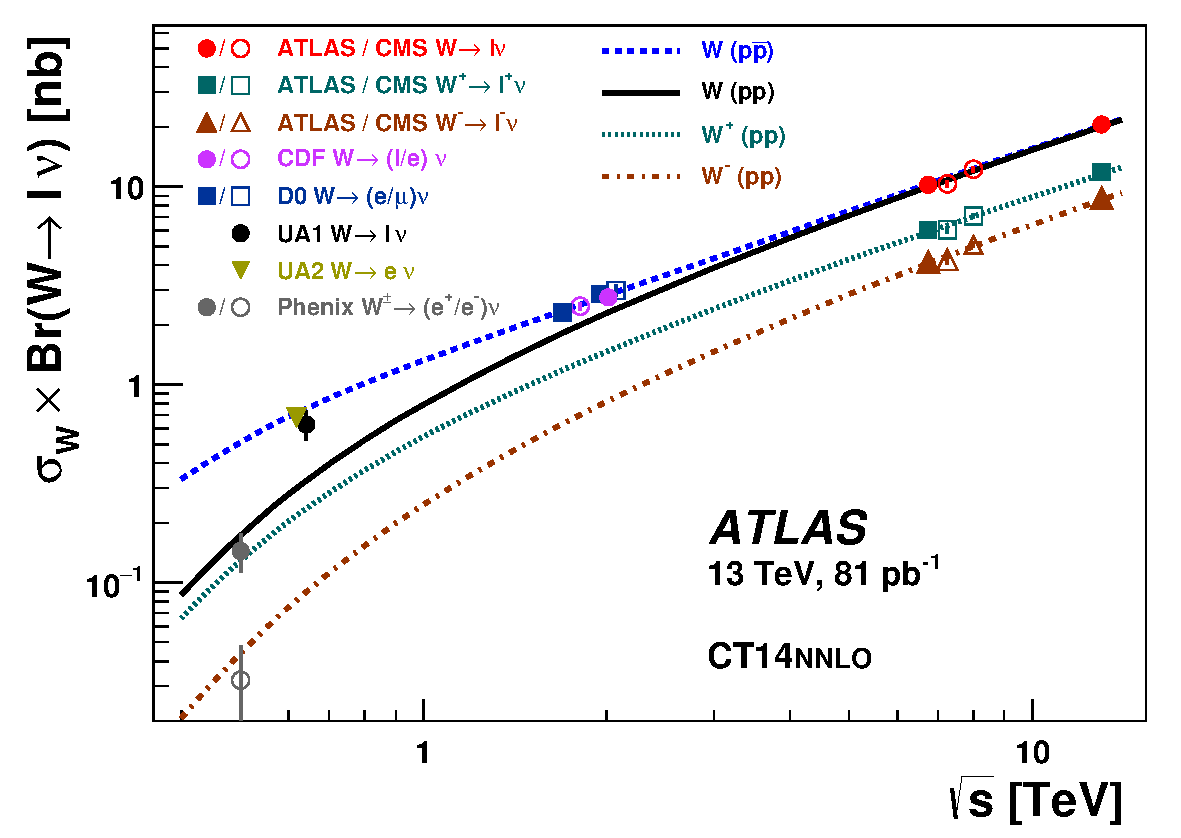
\includegraphics[width=0.7\linewidth]{Theory/Wcs.pdf} \\ a)}

\caption{The measured values of $\sigma_{W \to l\nu}$ for $W^+$, $W^-$ and  their sum compared to the theoretical predictions based on NNLO QCD calculations. The ATLAS results are shown for the combined electron-muon channel only. The predictions and previous measurements are shown for both proton-proton and proton-antiproton colliders as a function of $\sqrt{s}$. The data points at the various energies are staggered to improve readability. All data points are displayed with their total uncertainty. The calculations were performed with the program FEWZ using the CT14nnlo parton density function parametrisation. The theoretical uncertainties on the cross-section predictions are not shown. Taken from \cite{a13TeV}}
\label{fig:Wcs}
\end{figure}

\begin{figure}[!tbp]
\center{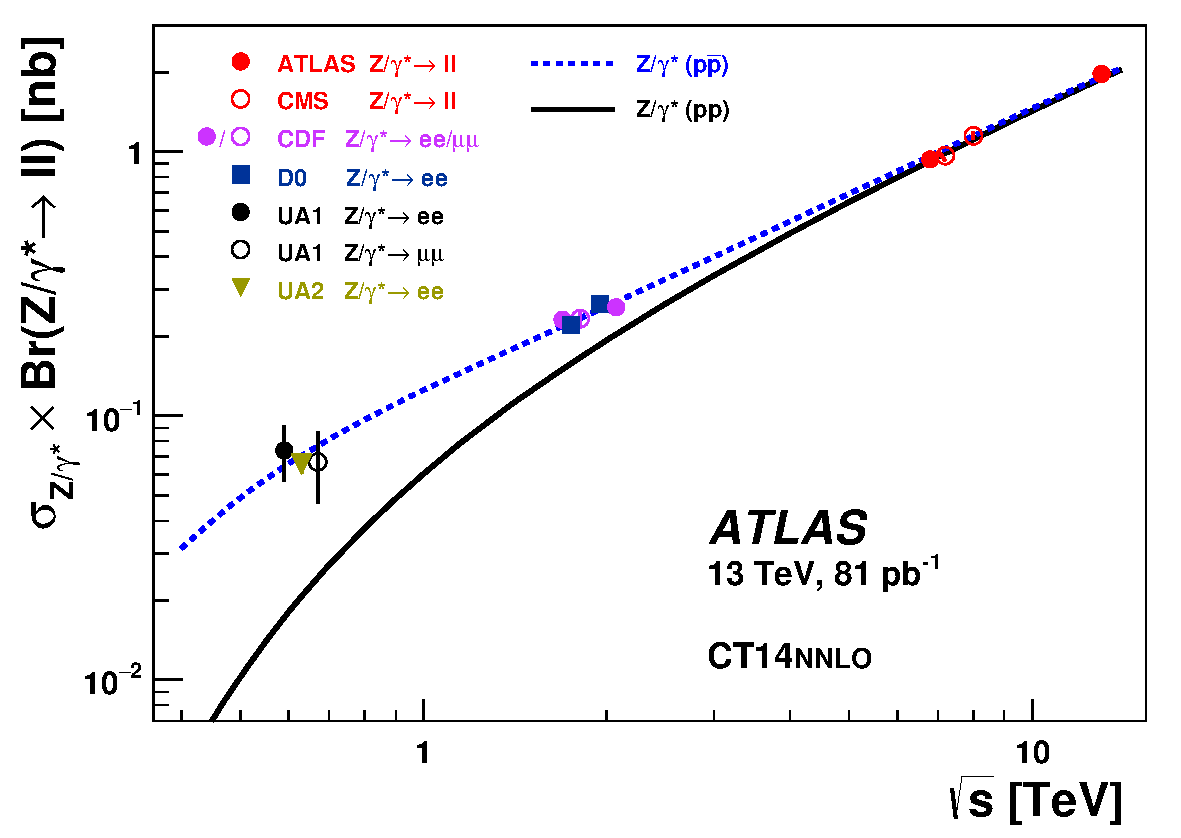
\includegraphics[width=0.7\linewidth]{Theory/Zcs.pdf} \\ b)}
\caption{The measured values of $\sigma_{Z \to ll}$ for Z-boson compared to the theoretical predictions based on NNLO QCD calculations. The ATLAS results are shown for the combined electron-muon channel only. The predictions and previous measurements are shown for both proton-proton and proton-antiproton colliders as a function of $\sqrt{s}$. The data points at the various energies are staggered to improve readability. All data points are displayed with their total uncertainty. The calculations were performed with the program FEWZ using the CT14nnlo parton density function parametrisation. The theoretical uncertainties on the cross-section predictions are not shown. Taken from \cite{a13TeV}}
\label{fig:Zcs}
\end{figure}

